\chapter{Future work and system maturation}
\label{chap:future-work}

The results presented in Chapter \ref{chap:experimental-results} demonstrated that geometry-driven stereo reconstruction provides a viable solution for three-dimensional tether observation under low-texture conditions where conventional photogrammetric methods fail. The experimental validation established the feasibility of recovering tether geometry through geometric continuity, radiometric localization, and constrained stereo correspondence.
\\\\
Despite these encouraging results, several opportunities remain for improving reconstruction robustness, increasing operational autonomy, and advancing the system toward a flight-ready implementation. The observations obtained during testing identified specific challenges related to topological ambiguities, temporal consistency, assessment of reconstruction confidence, and onboard deployment constraints.

This chapter outlines a roadmap for the proposed framework's maturation, as shown in Figure \ref{fig:figure7.1}. The discussion focuses on algorithmic enhancements for challenging observation scenarios, the integration of targeted AI-assisted perception tools, the hardware transition toward flight-compatible architectures, and the long-term evolution of the system into an operational tether-monitoring instrument for future space missions.

\begin{figure}[!ht]
    \centering
    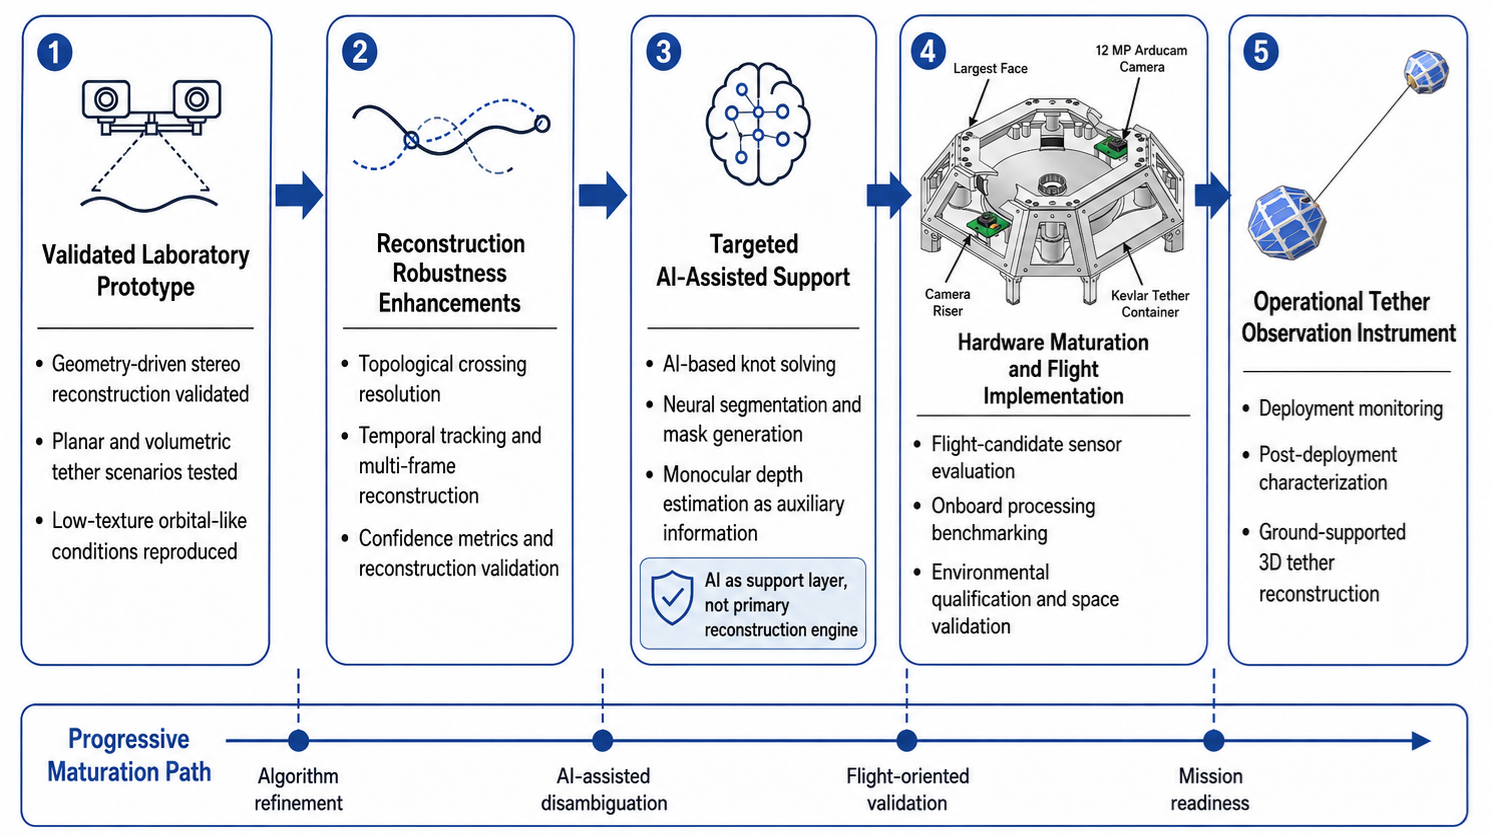
\includegraphics[width=\textwidth]{Images/Figure 7.1.png}
    \caption[Technology maturation roadmap for the LINKU stereo vision system.]{Technology maturation roadmap for the LINKU stereo vision system, showing the progression from laboratory validation toward a flight-compatible tether observation instrument.}
    \label{fig:figure7.1}
\end{figure}

\section{Reconstruction robustness enhancements}

The geometry-driven reconstruction framework successfully recovered tether geometries under the experimental conditions evaluated in this work. However, several opportunities for improvement were identified during testing, particularly in scenarios involving complex tether configurations, partial occlusions, and ambiguous geometric interpretations, as illustrated in Figure \ref{fig:figure7.2}. The following developments are proposed to increase reconstruction robustness while preserving the physical interpretability of the current methodology.

\begin{figure}[!ht]
    \centering
    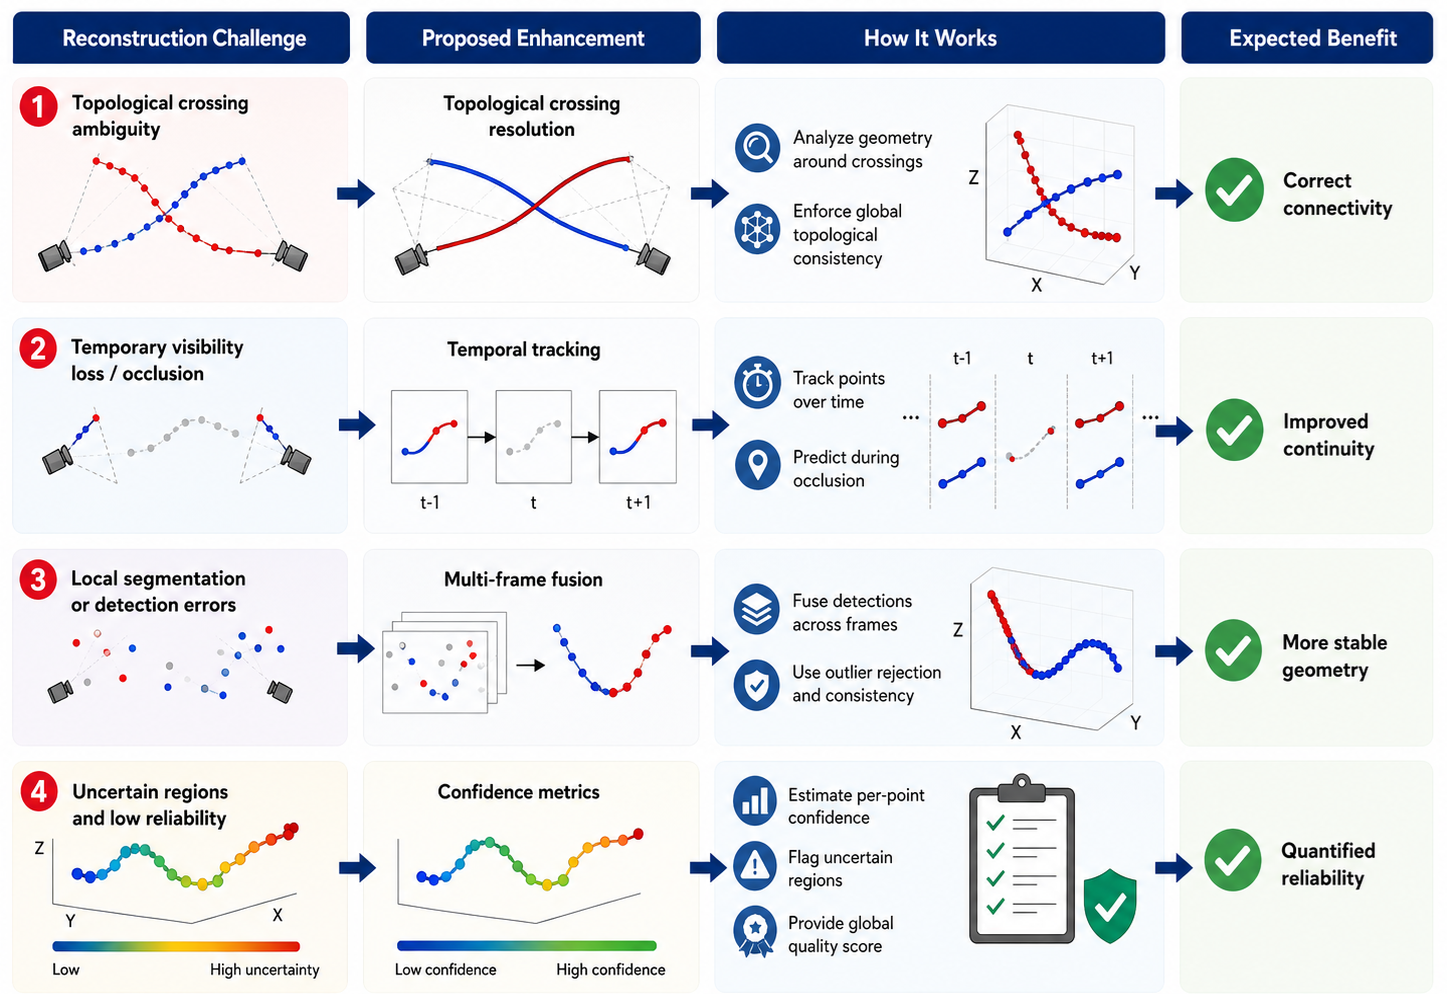
\includegraphics[width=\textwidth]{Images/Figure 7.2.png}
    \caption[Proposed robustness enhancements for the geometry-driven reconstruction framework.]{Proposed robustness enhancements for the geometry-driven reconstruction framework, including topological crossing resolution, temporal tracking, multi-frame reconstruction, and confidence-based validation.}
    \label{fig:figure7.2}
\end{figure}

\subsection{Topological crossing resolution}

One of the principal challenges identified during the experimental evaluation was the presence of topological crossings, where multiple tether segments overlap within the image plane. Although such events did not prevent reconstruction of the overall tether geometry, they introduced localized ambiguities regarding the true connectivity of the observed structure.
\\\\
Future work should focus on incorporating dedicated crossing-resolution strategies that can distinguish foreground and background tether branches. One possible approach is to integrate disparity-consistency checks, in which local depth information from stereo correspondence is used to determine the most physically plausible continuation path through an intersection. This would allow the reconstruction process to maintain geometric continuity even in highly entangled tether configurations.
\\\\
The development of robust topological reasoning capabilities is expected to improve reconstruction reliability during non-nominal deployment events, including slack tether motion, partial self-intersections, and dynamic oscillatory behavior.

\subsection{Temporal tracking and multi-frame reconstruction}

The current framework processes each stereo pair independently. While this approach simplifies implementation and validation, it does not exploit the temporal continuity naturally present in image sequences.
\\\\
Future implementations should incorporate temporal tracking mechanisms that propagate geometric information between consecutive frames. By using previously reconstructed tether trajectories as priors, the system could improve correspondence stability, reduce sensitivity to transient image artifacts, and assist in resolving topological ambiguities.
\\\\
Multi-frame reconstruction techniques may also improve robustness when portions of the tether are temporarily obscured by glare, motion blur, or partial occlusion. The use of temporal consistency constraints would enable the reconstruction process to recover missing information from neighboring observations rather than relying exclusively on a single image pair.

\subsection{Confidence metrics and reconstruction validation}

Future operational implementations will require quantitative indicators to assess reconstruction quality in the absence of external ground-truth references. Such metrics are particularly important for autonomous spaceborne systems, where manual verification of every reconstructed frame is impractical.
\\\\
A promising approach involves monitoring the consistency of stereo reprojection throughout the reconstruction process. Deviations between observed image locations and reconstructed projections can provide a direct measure of geometric reliability. Additional indicators may include correspondence density, centerline continuity, disparity consistency, and temporal stability across consecutive frames.
\\\\
The integration of confidence metrics would enable the system to associate each reconstructed tether segment with a quantitative quality estimate. These metrics could be incorporated into telemetry products, providing mission operators with objective indicators of reconstruction reliability and facilitating autonomous decision-making during long-duration tether observation campaigns.

\section{AI-assisted perception and topology analysis}

The exploratory assessment presented in Chapter \ref{chap:experimental-results} indicated that current generative AI methods are not suitable as primary reconstruction engines for scientific tether observation. However, the same assessment revealed several perception-oriented tasks in which AI could significantly enhance the robustness of the geometry-driven framework without compromising physical interpretability.
\\\\
Future AI integration should therefore focus on targeted assistance rather than end-to-end reconstruction. Under this strategy, geometric reconstruction remains responsible for generating scientifically traceable three-dimensional measurements, as specified in Figure \ref{fig:figure7.3}, while AI modules provide support in situations involving ambiguity, image degradation, or complex scene interpretation.
\newpage
\clearpage

\begin{figure}[!ht]
    \centering
    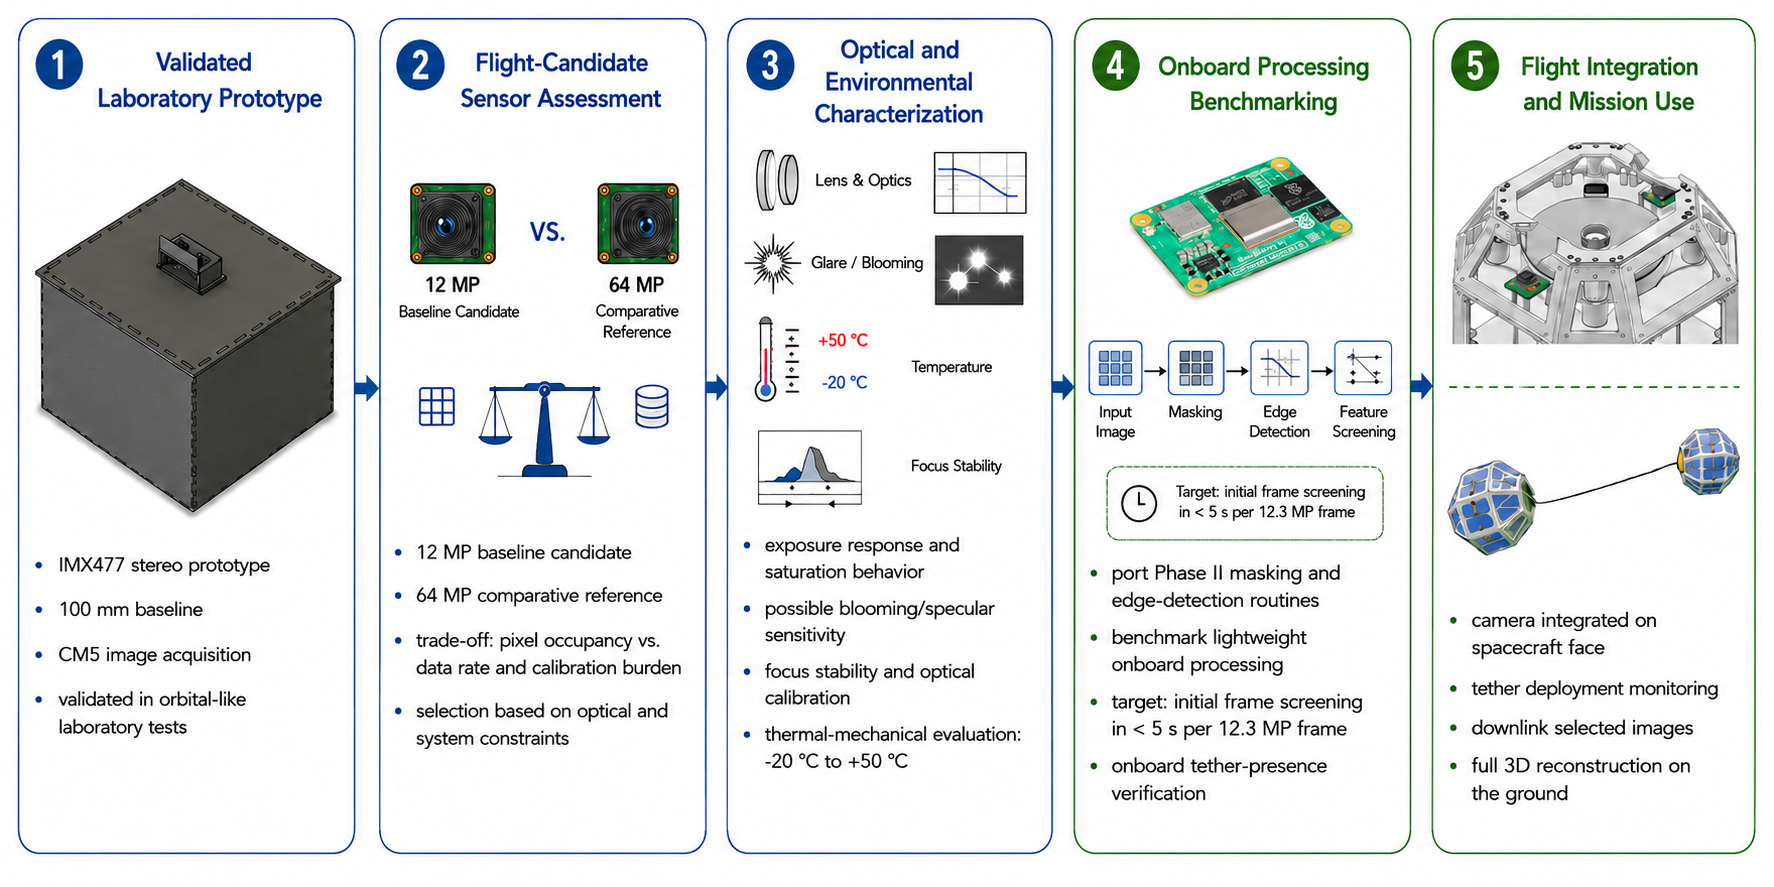
\includegraphics[width=\textwidth]{Images/Figure 7.3.png}
    \caption[Targeted AI assistance within the geometry-driven reconstruction pipeline.]{Targeted AI assistance within the geometry-driven reconstruction pipeline. AI modules are proposed as support tools for masking, knot solving, and ambiguity resolution, while the final reconstruction remains constrained by stereo geometry.}
    \label{fig:figure7.3}
\end{figure}

\subsection{AI-assisted wire path tracking (including knot solving)}

Topological crossings are among the most challenging scenarios for tether reconstruction because multiple physically distinct tether segments may project onto the same image region. Although geometric constraints and stereo correspondence can resolve many of these cases, highly entangled configurations may still produce ambiguous interpretations.
\\\\
This capability is treated as a single AI component together with ordinary path tracking, not as a separate knot-solving module, because both tasks require exactly the same decision: given a segmented thread image, choose the correct continuation at each point where more than one is geometrically possible. An untangled thread simply has few or no such points, while a knotted one has many; the same trained model is applicable to both. Chapter \ref{chap:experimental-processing-approaches} (Section \ref{sec:Geometry-driven stereo reconstruction}, Figure \ref{fig:ai-proposed-tracker}) proposes a concrete architecture for this component: it reuses the branch-point search already implemented in the classical tracker and replaces only the local scoring rule, which is currently a fixed hand-tuned formula, with one learned from operator-verified paths.
\\\\
This design offers two advantages over a general-purpose neural reconstruction module. First, it minimizes computational requirements by restricting learned inference to a single scoring decision at each branch point rather than processing the full image. Second, it preserves the interpretability of the overall reconstruction process, since the search structure, backtracking behavior, and downstream stereo matching remain exactly as validated in Chapter \ref{chap:experimental-results}; only the local weighting of already-physical features (direction continuity, thickness continuity, centeredness) becomes learned instead of hand-tuned.
\\\\
Reaching this point in practice requires two further steps beyond the current state: growing the path dataset from its present size (1 stereo sample) to the 30--100 samples typically needed for a small classifier of this kind, and building the offline tooling that converts a verified path into labeled (candidate-features, chosen-branch) training examples at each branch point along it.

\subsection{Neural segmentation and mask generation}

Accurate tether extraction remains a critical prerequisite for all subsequent reconstruction stages. A first implementation of this capability already exists: a pixel-level Random Forest classifier (Chapter \ref{chap:experimental-processing-approaches}, Section \ref{sec:Geometry-driven stereo reconstruction}) trained on 6 manually labeled stereo pairs, selectable as an alternative to manual intensity-based thresholding. While this approach proved effective under the experimental conditions evaluated in this work, future operational environments may introduce more challenging illumination scenarios.
\\\\
Examples include severe specular reflections, sensor saturation, non-uniform illumination, partial shadows, and varying background radiometric conditions. Under such circumstances, both the current threshold-based and Random-Forest-based segmentation may become less reliable, and the small training set used so far has not yet been validated on a held-out set.
\\\\
Future research should therefore evaluate lightweight neural segmentation architectures that can generate robust tether masks under adverse imaging conditions, as a further iteration of the same component. Models derived from U-Net or similar encoder-decoder architectures are promising candidates because they can learn object-specific features while maintaining relatively low computational complexity, and could be trained on the same growing dataset already being collected.
\\\\
Importantly, the role of these models would be limited to image preprocessing. The resulting binary masks would continue to be processed by the geometry-driven reconstruction pipeline, preserving the physical basis of the three-dimensional reconstruction process.

\subsection{Monocular depth estimation as auxiliary information}

Although stereo vision remains the primary source of depth information in the proposed framework, future systems may benefit from complementary depth estimation techniques that provide additional geometric cues.
\\\\
Recent advances in foundation models for monocular depth estimation have demonstrated the ability to infer relative depth relationships from single images. While these estimates do not generally provide metric accuracy comparable to stereo triangulation, they can supply useful contextual information regarding foreground-background ordering and local geometric structure.
\\\\
Future work should investigate whether monocular depth estimation can serve as an auxiliary source of information during reconstruction. Potential applications include resolving depth ambiguities at topological crossings, validating stereo correspondence hypotheses, and improving robustness when stereo matching performance is degraded by glare, motion blur, or partial occlusion.
\\\\
Under this approach, monocular depth estimation would not replace stereo reconstruction. Instead, it would serve as a secondary information layer that assists the geometry-driven framework when direct geometric measurements become uncertain.

\section{Hardware maturation and flight implementation}

The experimental validation presented in Chapters \ref{chap:experimental-setup-hardware-config} and \ref{chap:experimental-results} demonstrated the feasibility of geometry-driven tether reconstruction using a laboratory-scale prototype based on commercial imaging hardware, as depicted in Figure \ref{fig:figure7.4}. The next stage of development focuses on transitioning from proof-of-concept validation toward a flight-compatible implementation capable of operating under the environmental, computational, and operational constraints of a space mission.

\begin{figure}[!ht]
    \centering
    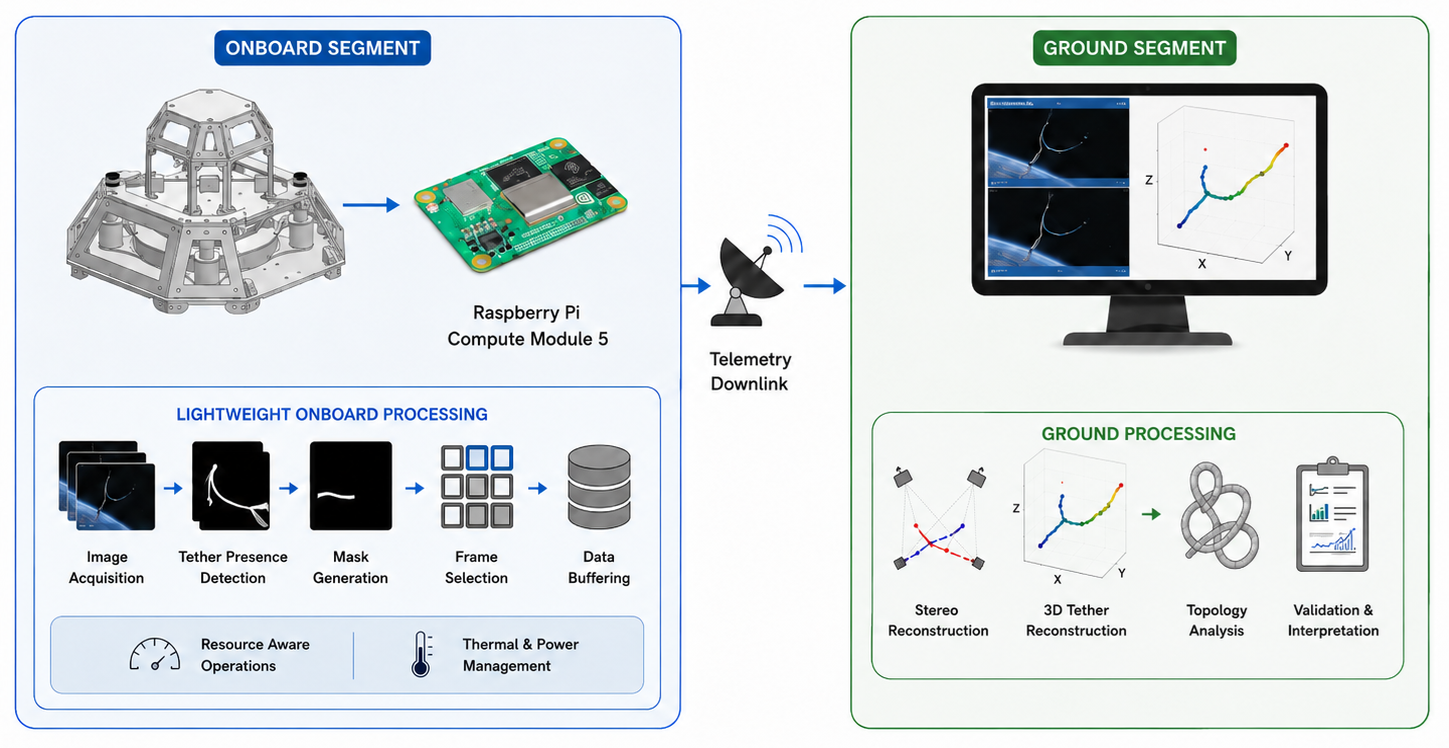
\includegraphics[width=\textwidth]{Images/Figure 7.4.png}
    \caption[Flight implementation architecture for the LINKU stereo vision system.]{Proposed flight implementation architecture, separating lightweight onboard image-processing tasks from full three-dimensional reconstruction and topology analysis performed on the ground segment.}
    \label{fig:figure7.4}
\end{figure}


Future work should therefore address three complementary areas: sensor selection and characterization, onboard processing validation, and environmental qualification of the complete imaging system.

\subsection{Flight-candidate sensor evaluation}

The observability analysis presented in Chapter 3 demonstrated that image resolution directly influences tether detectability by increasing the projected tether occupancy in the image plane. However, the analysis also showed that higher pixel counts alone do not eliminate the sub-pixel observation regime encountered at long distances.
\\\\
Consequently, future sensor selection should not be based exclusively on spatial resolution. Instead, a comprehensive trade-off analysis should consider optical performance, sensitivity, dynamic range, data throughput, processing requirements, and environmental robustness.
\\\\
The IMX477-based architecture remains a suitable baseline for continued development because it supported all experimental validation activities performed in this work and offers interchangeable optics for controlled testing. Alternative high-resolution sensors may provide improved long-range observability but impose additional demands on storage, bandwidth, calibration, and onboard processing.
\\\\
Future characterization campaigns should evaluate:
\begin{itemize}
    \item Radiometric sensitivity and signal-to-noise ratio.
    \item Dynamic range under high-contrast illumination.
    \item Susceptibility to saturation and blooming effects.
    \item Optical stability under temperature variations.
    \item Calibration repeatability and long-term performance.
\end{itemize}

These measurements will provide the information required to establish a flight-candidate imaging architecture aligned with the observation requirements of future tether missions.

\subsection{Onboard processing benchmarking}

The reconstruction pipeline developed in this work was validated using ground-based processing resources. Future mission implementations will require partial onboard execution to reduce communication bandwidth and support autonomous operation.
\\\\
A first maturation step consists of porting the preprocessing stages of the geometry-driven framework to a representative flight-computing platform such as the Raspberry Pi Compute Module 5. Particular attention should be given to image acquisition, tether masking, centerline extraction, and preliminary feature validation, as these stages determine whether useful tether information is present within the acquired image.
\\\\
Benchmarking activities should quantify:

\begin{itemize}
    \item Processing time per image.
    \item Memory utilization.
    \item Processor workload.
    \item Power consumption.
    \item Maximum sustainable image acquisition rate.
\end{itemize}

These measurements will establish whether low-level tether detection can be performed onboard before transmitting reduced data products or selected image subsets to the ground segment. Such an approach could significantly reduce downlink requirements while preserving scientifically relevant information.
\\\\
Longer-term developments may also evaluate the feasibility of performing partial stereo correspondence estimation onboard, reserving full three-dimensional reconstruction for ground-based processing systems.

\subsection{Environmental qualification and space validation}

Although the current prototype successfully demonstrated the proposed reconstruction methodology, its operational performance has not yet been evaluated under representative space environmental conditions.
\\\\
Future work should therefore include environmental characterization campaigns addressing the principal factors expected during orbital operation. These include thermal variations, vibration exposure, launch-induced mechanical loads, illumination variability, and long-duration operational stability.
\\\\
Recommended qualification activities include:

\begin{itemize}
    \item Thermal cycling tests to evaluate focus stability and geometric calibration drift.
    \item Vibration testing to verify structural integrity of the camera assembly.
    \item Optical characterization under varying illumination geometries.
    \item Long-duration operational testing to assess calibration stability over time.
    \item End-to-end validation using representative deployment sequences and observation distances.
\end{itemize}

Beyond laboratory qualification, the ultimate maturation objective is the demonstration of tether observation under operationally relevant conditions. Potential intermediate validation platforms include drone-based deployments, high-altitude balloon experiments, and dedicated in-orbit technology demonstrations.
\\\\
Completion of these activities would increase the Technology Readiness Level (TRL) of the system and provide the experimental evidence required to support integration into future tether deployment, inspection, and monitoring missions.

\section{Path toward operational tether observation missions}

The results presented throughout this work lay the foundation for developing future tether observation systems that support deployment monitoring, structural characterization, and operational diagnostics in space environments. The proposed geometry-driven framework demonstrated that reliable tether reconstruction can be achieved without conventional texture-based photogrammetric techniques, enabling observation of thin, elongated structures that would otherwise be difficult to characterize with traditional computer vision methods.
\\\\
The next stage of system maturation involves the transition from laboratory validation to operational deployment scenarios. This process requires the progressive integration of the algorithmic, sensing, and processing developments discussed in Sections 7.1 through 7.3. In particular, improvements in topological ambiguity resolution, temporal tracking, onboard processing, and environmental qualification will increase the robustness and autonomy required for flight operations.
\\\\
Future mission architectures may employ the proposed framework in several operational roles, including:

\begin{itemize}
    \item Tether deployment monitoring, providing real-time assessment of deployment geometry, trajectory evolution, and anomaly detection.
    \item Structural shape reconstruction, enabling characterization of tether curvature, oscillatory motion, and dynamic behavior during mission operations.
    \item Health and status assessment, supporting the identification of abnormal deployment conditions, entanglements, excessive slack, or unexpected structural deformations.
    \item Post-deployment analysis that allows reconstruction of tether geometry from stored image sequences for engineering evaluation and mission performance assessment.
\end{itemize}

Beyond tether-specific applications, the methodology may also be extended to other elongated or low-texture structures encountered in space systems, including deployable booms, flexible appendages, cables, and lightweight structural elements. The underlying principles of geometric continuity, radiometric localization, and constrained stereo reconstruction are not limited to tethered observations and may therefore support a broader class of spaceborne inspection and monitoring tasks.
\\\\
From a mission perspective, the proposed architecture enables a distributed processing strategy in which computationally efficient detection and validation functions are executed onboard, while high-fidelity three-dimensional reconstruction is performed on the ground segment when required. This approach balances onboard resource constraints with the need for accurate geometric characterization and is consistent with the operational concepts commonly employed in modern small satellite missions.
\\\\
Ultimately, the maturation pathway described in this chapter provides a practical roadmap for evolving the current proof-of-concept implementation into a flight-capable tether observation instrument. By combining physics-based reconstruction, targeted AI assistance, and flight-oriented hardware validation, the framework offers a scalable approach for future orbital tether missions and contributes to the broader objective of improving autonomous monitoring capabilities for next-generation space systems.
